% Name: Spring and mass
% Description: A mass on a frictionless floor, tied to a wall by a spring and pulled a distance x from where the spring is at rest.
% Tags: spring, harmonic oscillator, Hooke's law, oscillation

\usetikzlibrary{arrows.meta, decorations.pathmorphing, patterns}

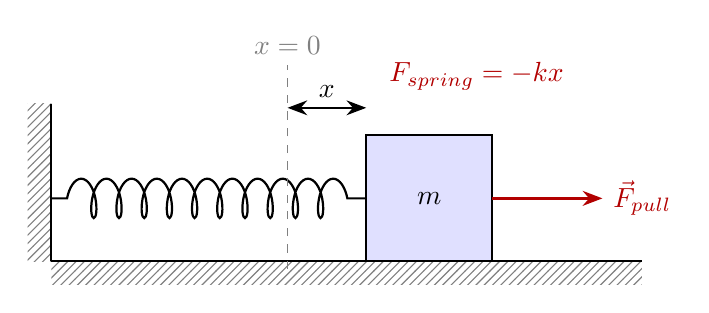
\begin{tikzpicture}[>={Stealth[length=2.5mm]}]
  \fill[pattern=north east lines, pattern color=gray] (-0.3,0) rectangle (0,2);
  \draw[thick] (0,0) -- (0,2);
  \fill[pattern=north east lines, pattern color=gray] (0,-0.3) rectangle (7.5,0);
  \draw[thick] (0,0) -- (7.5,0);
  \draw[thick, decorate, decoration={coil, aspect=0.4, segment length=3.2mm, amplitude=2.5mm, pre length=2mm, post length=2mm}] (0,0.8) -- (4,0.8);
  \draw[thick, fill=blue!12] (4,0) rectangle (5.6,1.6) node[midway] {$m$};
  \draw[dashed, gray] (3,-0.1) -- (3,2.5) node[above] {$x = 0$};
  \draw[<->, thick] (3,1.95) -- node[above] {$x$} (4,1.95);
  \draw[->, very thick, red!70!black] (5.6,0.8) -- ++(1.4,0) node[right] {$\vec{F}_{\text{pull}}$};
  \node[red!70!black] at (5.4,2.35) {$F_{\text{spring}} = -kx$};
\end{tikzpicture}
